%
%  untitled
%
%  Created by Dean Freestone on 2010-07-06.
%  Copyright (c) 2010 . All rights reserved.
%
\documentclass[]{article}

% Use utf-8 encoding for foreign characters
\usepackage[utf8]{inputenc}

% Setup for fullpage use
\usepackage{fullpage}

% Uncomment some of the following if you use the features
%
% Running Headers and footers
%\usepackage{fancyhdr}

% Multipart figures
%\usepackage{subfigure}

% More symbols
%\usepackage{amsmath}
%\usepackage{amssymb}
%\usepackage{latexsym}

% Surround parts of graphics with box
\usepackage{boxedminipage}

% Package for including code in the document
\usepackage{listings}

% If you want to generate a toc for each chapter (use with book)
\usepackage{minitoc}

% This is now the recommended way for checking for PDFLaTeX:
\usepackage{ifpdf}

\usepackage{amsmath,amssymb,amsfonts,epsfig} % Typical maths resource packages

%\newif\ifpdf
%\ifx\pdfoutput\undefined
%\pdffalse % we are not running PDFLaTeX
%\else
%\pdfoutput=1 % we are running PDFLaTeX
%\pdftrue
%\fi

\ifpdf
\usepackage[pdftex]{graphicx}
\else
\usepackage{graphicx}
\fi
\title{Patient-Specific Neural Field Model}
\author{Parham Aram, Dean Freestone, Kenneth Scerri, Michael Dewar,\\
 Jacob Donoghue, Sydney Cash, David Grayden and Visakan Kadirkamanathan  }

\date{2010-07-06}

\begin{document}

\ifpdf
\DeclareGraphicsExtensions{.pdf, .jpg, .tif}
\else
\DeclareGraphicsExtensions{.eps, .jpg}
\fi

\maketitle


\begin{abstract}
	
	\begin{itemize}
		\item Background
		\item Method
		\item Result
		\item Conclusion
	\end{itemize}
\end{abstract}

\section{Introduction}
\begin{itemize}
	\item Understanding of macroscopic neurodynamics
	\item Neural field model
	\item Improvements in electrode technology with great spatiotemporal resolution
\end{itemize}

\section{Method}

\subsection{Data Collection}
\begin{itemize}
	\item Show medical imaging
	\item Show LFP Data (background, seizure, post-seizure)
	\item Show spectral properties of LFPs
\end{itemize}

\begin{figure}[!ht]
\begin{center}
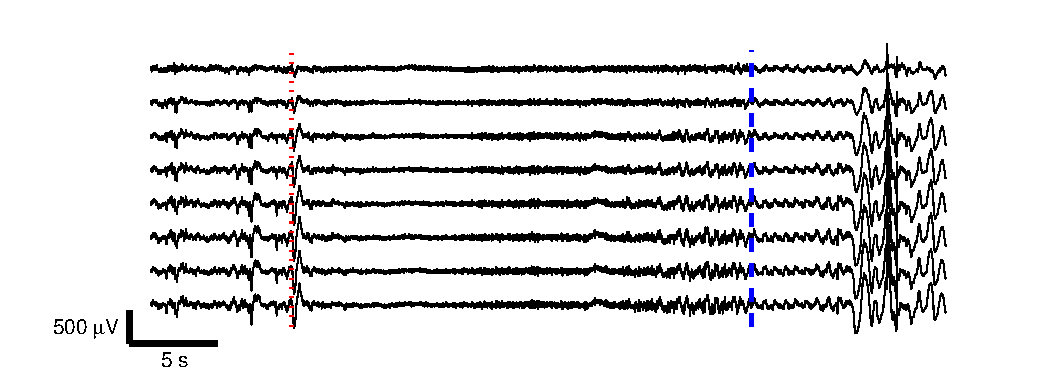
\includegraphics{./Figures/LFPs.eps}
\end{center}
\caption{{\bf Local Field Potentials}. Data recorded from the first five channels of the array. The red dotted line indicates the seizure onset and the blue dashed line indicates the seizure end.}
\label{fig:TimeSeries}
\end{figure}

\begin{figure}[!ht]
\begin{center}
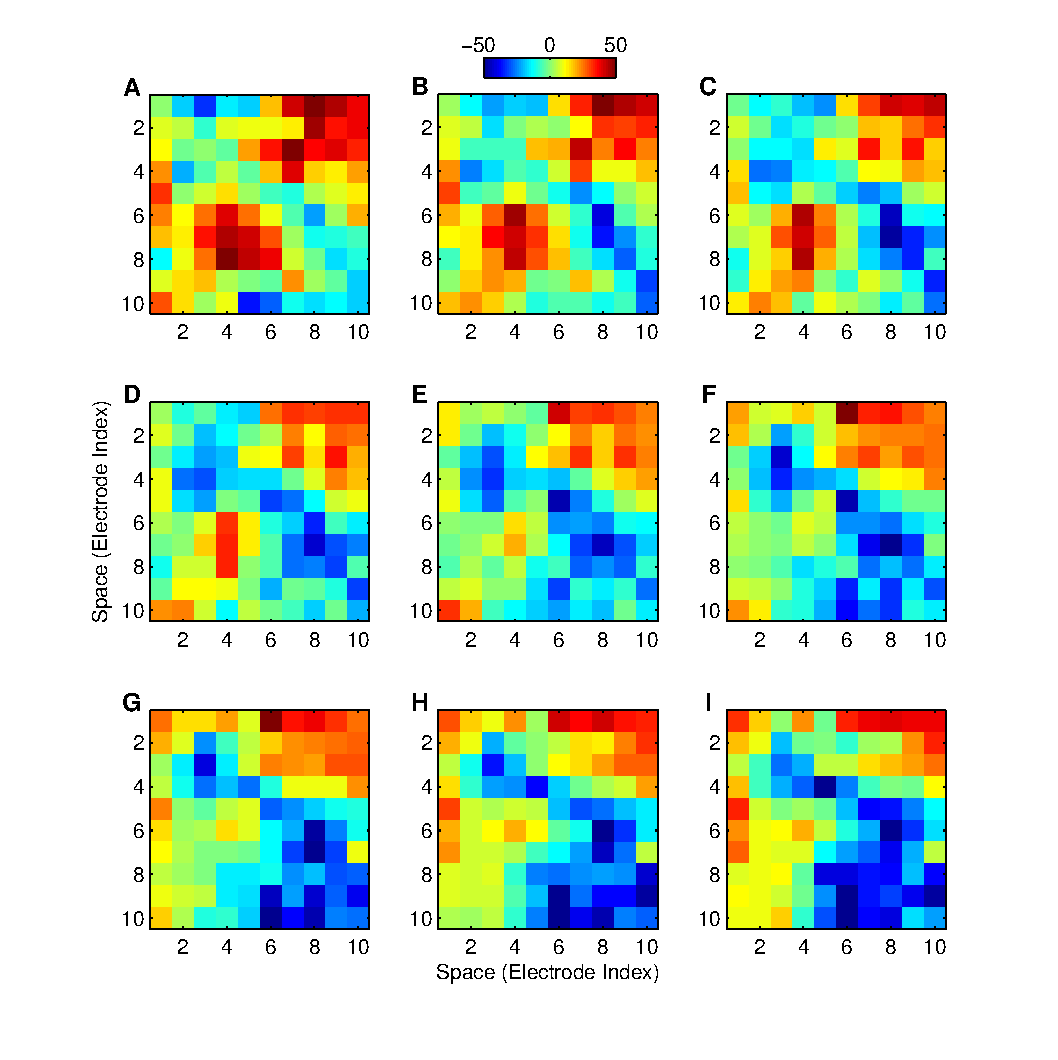
\includegraphics{./Figures/FieldObservations.eps}
\end{center}
\caption{{\bf Snap-shots of the spatial aspects of the observed field}. The snap-shots are ordered from A to I forming a consecutive sequence spaced 2.5~ms apart starting at 34.024s}
\label{fig:FieldObserations}
\end{figure}

\begin{figure}[!ht]
\begin{center}
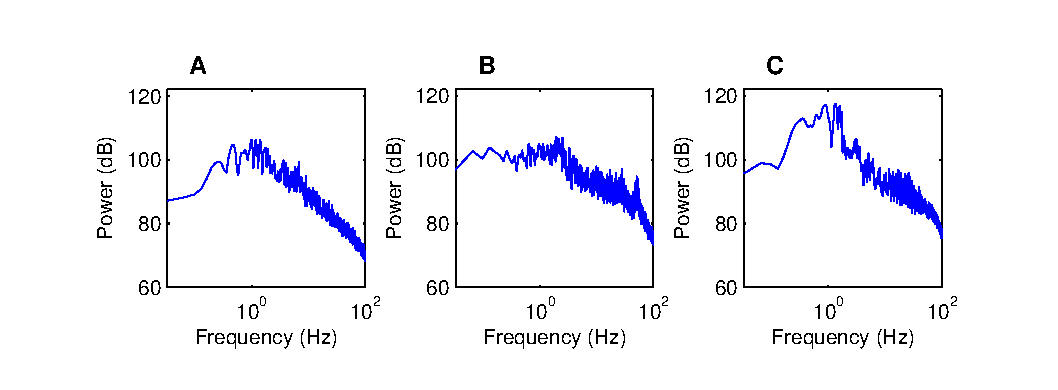
\includegraphics{./Figures/TemporalFreq.eps}
\end{center}
\caption{{\bf Spectra from local field potential recordings}. A. Pre-seizure observations. B. Seizure observations. C. Post-seizure observations.}
\label{fig:TemporalFreqObservation}
\end{figure}

\subsection{Frequency Analysis}
\begin{itemize}
	\item Create 2D FT of observations to estimate bandwidth
\end{itemize}

\begin{figure}[!ht]
\begin{center}
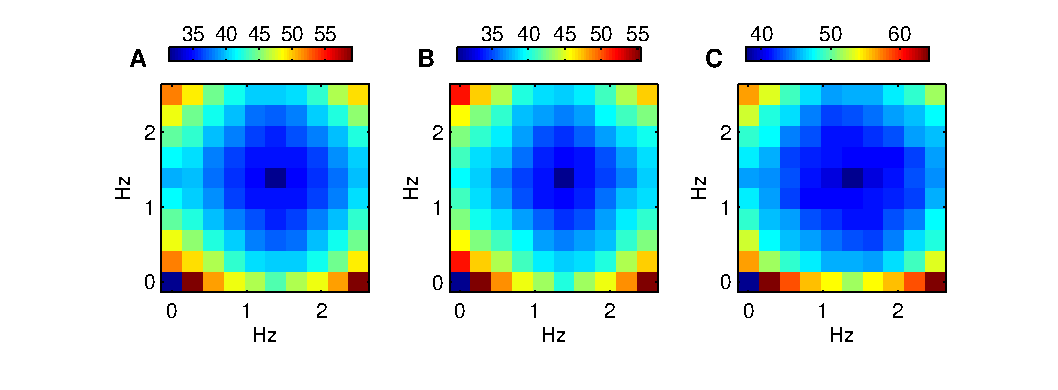
\includegraphics{./Figures/SpatialFreq.eps}
\end{center}
\caption{{\bf Spatial frequency analysis of the observed neural field}. A. Pre-seizure observations. B. Seizure observations. C. Post-seizure observations.}
\label{fig:SpatialFreqObservation}
\end{figure}

\begin{figure}[!ht]
\begin{center}
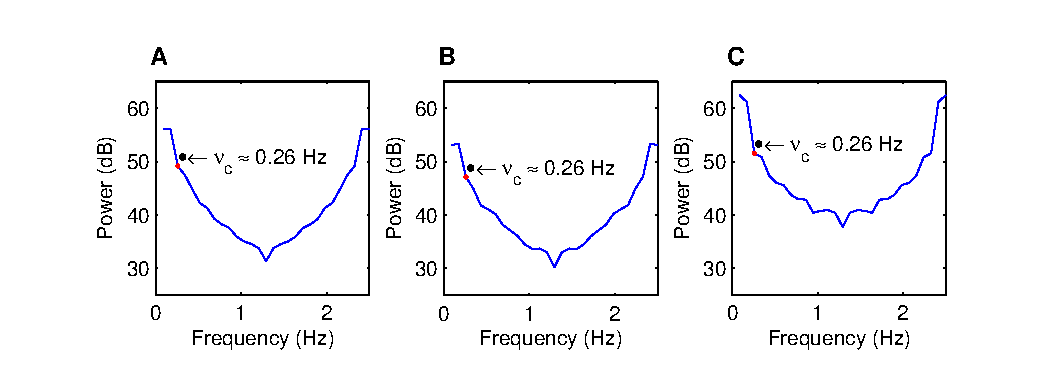
\includegraphics{./Figures/SpatialFreqCrossSection.eps}
\end{center}
\caption{{\bf Diagonal cross-section of the spatial frequency plots of the observed neural field}. A. Pre-seizure observations. B. Seizure observations. C. Post-seizure observations.}
\label{fig:SpatialFreqObservation}
\end{figure}

\subsection{Pre-processing}
\begin{itemize}
	\item Identification and removal of bad channels
	\item Common average reference (CAR) montage 
	\item Low-pass filter data, with cut-off at 100~Hz
	\item Decimate data from 30~kHz to 5~kHz temporal sampling
	\item Spatially interpolate missing data to facilitate spatial frequency analysis
\end{itemize}
\subsection{Estimation Algorithm}
\begin{itemize}
	\item Model
	\item URTSS
\end{itemize}

\section{Results}
\begin{itemize}
	\item Will show parameter distributions
	\item Will show parameter changes over time through the seizure
\end{itemize}

\section{Discussion}
\begin{itemize}
	\item  
\end{itemize}

\bibliographystyle{plain}
\bibliography{}
\end{document}
